\documentclass[main.tex]{subfiles}

% Quantum Circuits
\begin{document}

    Valentino Braitenberg (1926-2011) was an Italian neuroscientist and a synthetic psychologist. He spent most of his life doing experiments to understand how the animal nervous system works. He was also interested in building synthetic models of human or animal behaviour. He is well known for his book~\cite{braitenberg1986vehicles}. This book consists of a series of thought experiments about behaviours which can be expected of simple devices. All these thought experiments were inspired by animals and their nervous systems. He said ``when we analyse a mechanism, we tend to over-estimate its complexity".

    \textbf{Working of a Basic Braitenberg Vehicle:} These are simple vehicles consisting of actively driven wheels and sensors. The sensors are stimulated by some stimulus (light, temperature, sound, presence of certain chemicals etc). The rotation speed of the wheels is directly controlled by the two sensor data. Depending upon how many sensors and wheels are there and how the sensor data influences the wheel speed (either excitatory or inhibitor), Braitenberg vehicles have been divided into the following categories:

    \begin{enumerate}



        % Vehicle S1
        \begin{figure}[t]%
            \centering
            \subfloat[\centering Excitatory Signal]{{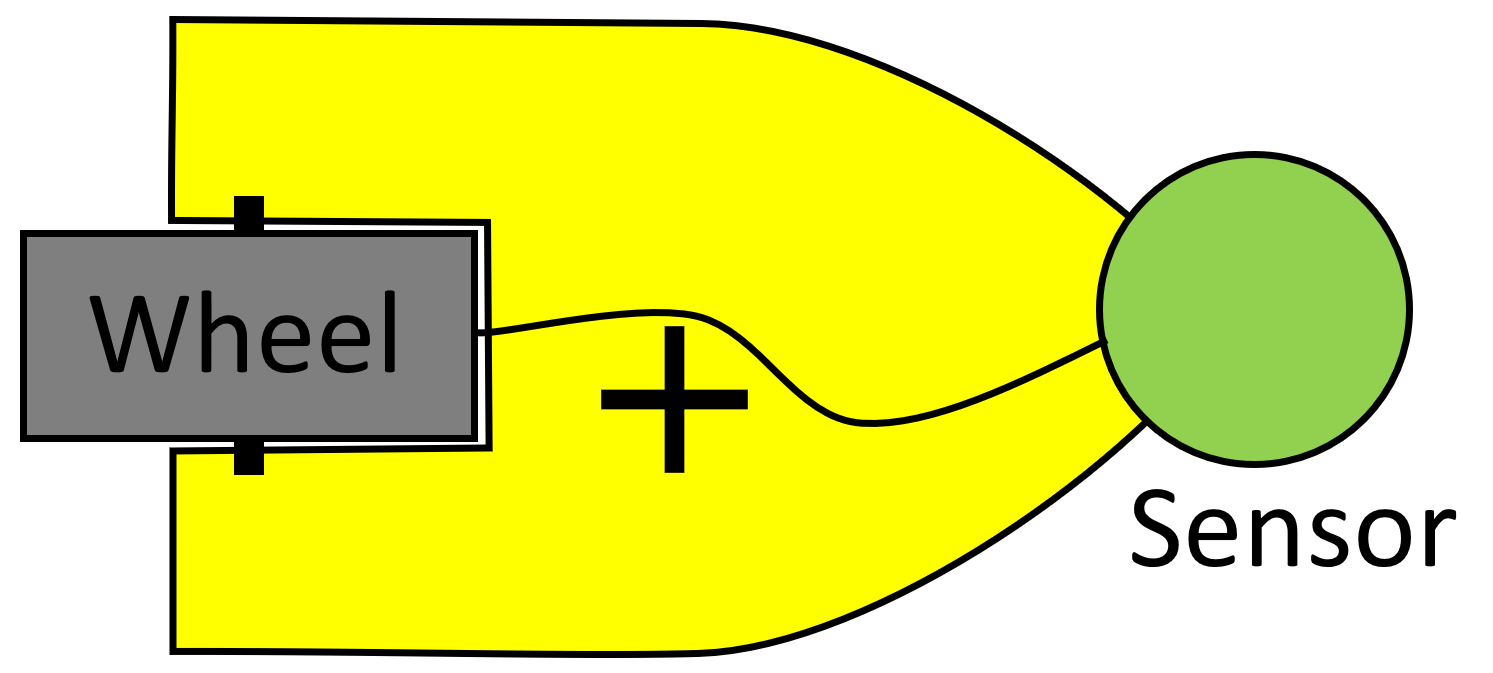
\includegraphics[width=5cm]{./images/1s_vehicle_p.png} }}%
            \qquad
            \subfloat[\centering Inhibitory Signal]{{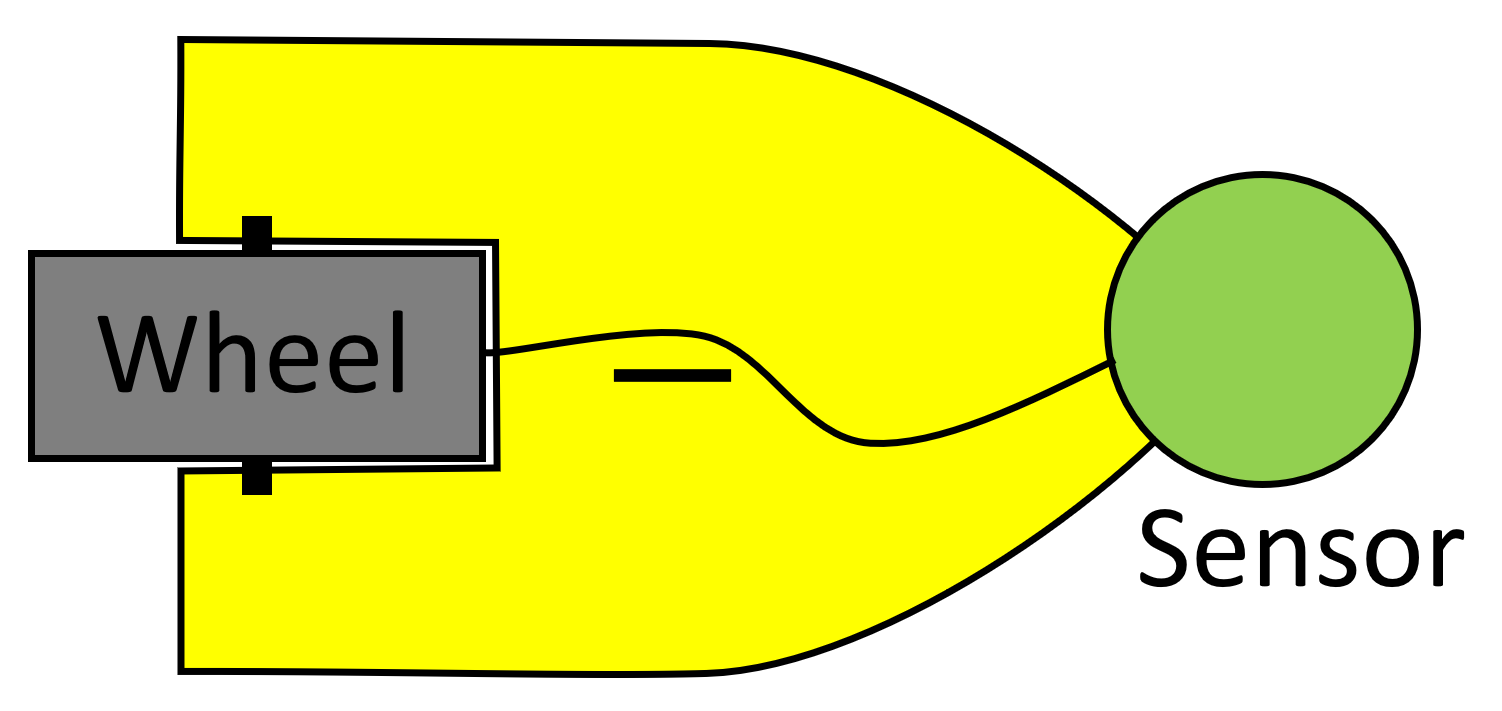
\includegraphics[width=5cm]{./images/1s_vehicle_m.png} }}%
            \caption{Braitenberg Vehicle Model 1}%
            \label{fig:vehicle1}%
        \end{figure}

        \item \textbf{Vehicle 1:} These vehicles (in Fig \ref{fig:vehicle1}) consist of a single sensor and a single wheel. These devices cannot change their directions. They move in a straight line. Now the sensor can either give an excitatory or an inhibitory signal to the wheel:

        \begin{itemize}
            \item \textbf{Excitatory Signal from Sensor:} Here, wheel speed is directly proportional to the strength of the stimulus. As the sensor senses more stimulus, (the stimulus is near) the wheel rotates faster; the vehicle gains speed. Thus, the speed of the vehicle is more when the vehicle is near the stimulus and the vehicle moves slowly when it is away from the stimulus. As a result, it spends less time near the source of stimulus and more time roaming away from it.
           \item \textbf{Inhibitory Signal from Sensor:} Here, wheel speed is inversely proportional to the strength of the stimulus. As the sensor senses more stimulus, the vehicle slows down. Thus, the devices gather around the source of stimulus.
        \end{itemize}




       % Vehicle S2
        \begin{figure}[b]%
            \centering
            \subfloat[\centering Uncrossed Connection]{{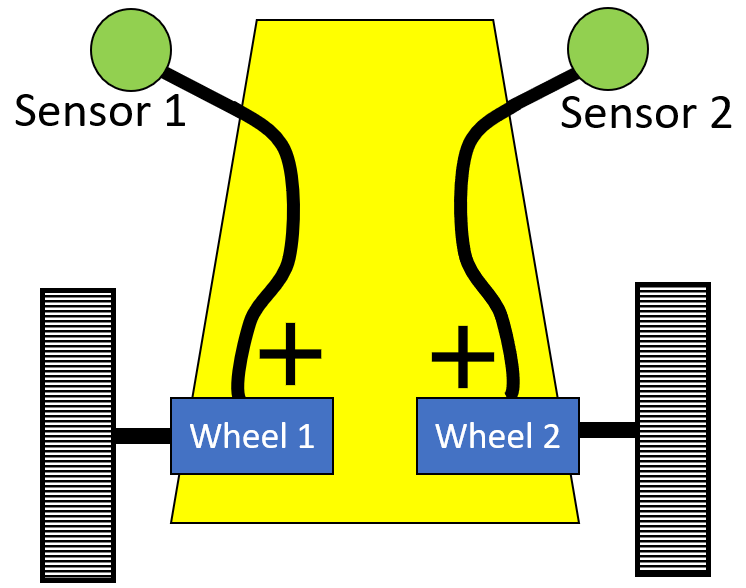
\includegraphics[width=5cm]{./images/2s_vehicle_d.png}}}%
            \qquad
            \subfloat[\centering Crossed Connection]{{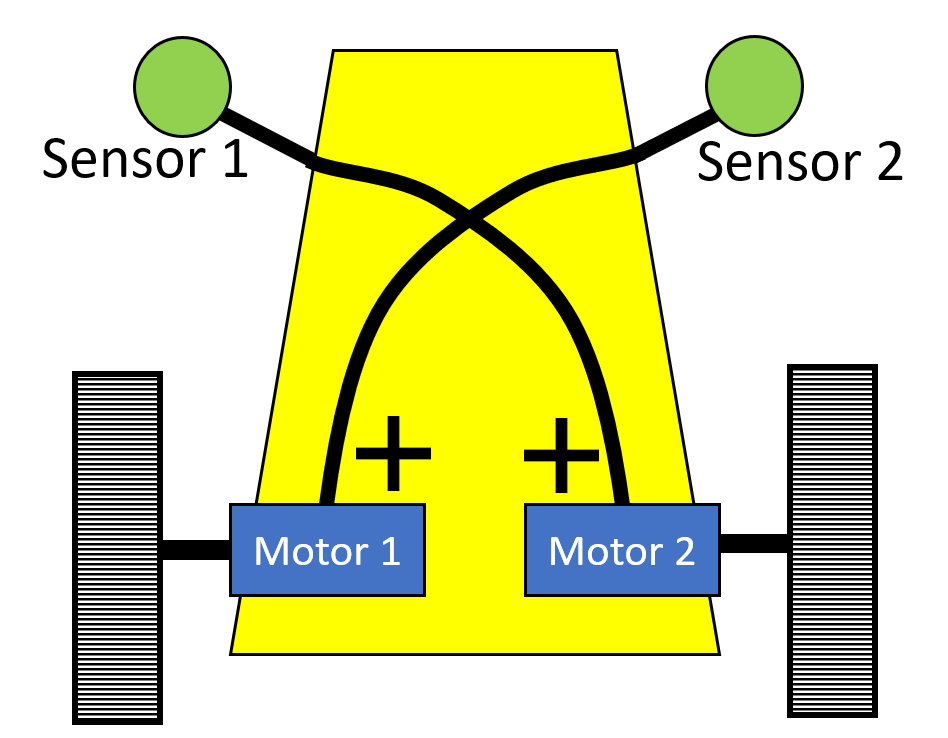
\includegraphics[width=5cm]{./images/2s_vehicle_c.png}}}%
            \caption{Braitenberg Vehicle Model 2}%
            \label{fig:vehicle2}%
        \end{figure}

        \item \textbf{Vehicle 2:} These vehicles (in Fig \ref{fig:vehicle2}) consist of two sensors and two wheels. Unlike Vehicle 1, they can move freely on a 2D plane. But here, the sensors can always give an excitatory signal to the wheels. They have been divided into 3 categories depending upon the connections:

        \begin{itemize}
            \item \textbf{Uncrossed connections (2a):} Here, the left sensor is attached to the left wheel and the right sensor is attached to the right wheel. Now, suppose a source of stimulus is present on the right side of the vehicle, the right sensor is stimulated more than the left one. Hence the right wheel rotates faster than the left wheel. Thus the vehicle turns left and goes away from the stimulus. \textbf{Inference:} The vehicle expresses \textbf{fear} from the cause of the stimulus.
            \item \textbf{Crossed connections (2b):} In this case, the left sensor is attached to the right wheel and the right sensor is attached to the left wheel. Now, to a stimulus on the right, the system responds by rotating the left wheel faster. It moves towards the stimulus. As it moves closer to the stimulus, its speed increases. Soon, the vehicle collides with the stimulus at great speed. \textbf{Inference:} The vehicle expresses \textbf{aggression/ hate} towards the cause of the stimulus.
            \item \textbf{Double connections (2c):} Here, both the sensors are connected to both the wheels. As both the wheels symultaneously recieve the same signal, this vehicle cannot turn (turning is achieved by different speed of the wheels). Thus, inspite of having a more complex connection, the vehicle is inferior to both 2a and 2b vehicles. \textbf{Inference:} More complex connections do not always give us to more complex functionality.
        \end{itemize}

    \end{enumerate}
    
    Braitenberg talked about a lot of other sorts of vehicles which show love, hatered, and many other behaviours. But this much discussion is enough for the purpose of this report. So, I will not go into the details of the other vehicles.

\end{document}
